\section{Introduction to the course}
\subsection{Course informations}
\textbf{Professor Marco Colombetti WebEx's room link:}\newline
\url{https://politecnicomilano.webex.com/meet/marco.colombetti}\newline
\newline
\textbf{Stuart Russell, Peter Norvig (2010). Artificial Intelligence: A modern approach, 3rd edition, Prentice-Hall/Pearson:}\newline
\url{../other/Artificial Intelligence: Artificial Intelligence A modern approach.pdf}\newline
The textbook is essential, because the slides and additional materials published on Beep will
not cover everything.\newline
\newline
\textbf{Professor's slides}:\newline
\url{../other/professor's slidesPart I - Introduction to the course.pdf}
\newline
\newline
\textbf{Lessons informations:}
\begin{center}
    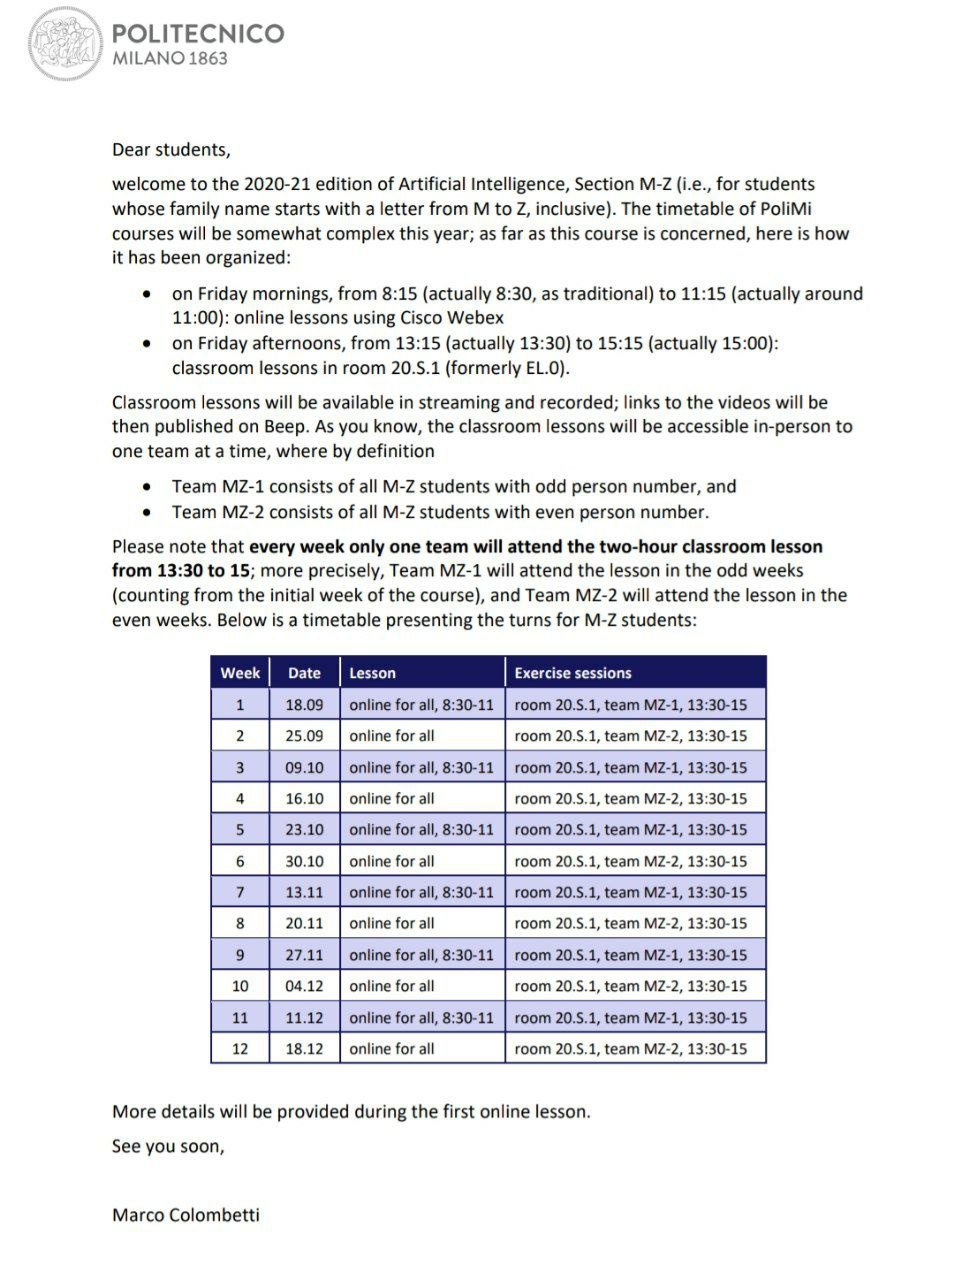
\includegraphics[height=17cm]{../other/schedule.jpg}
\end{center}
\ \newline
The course concerns \textbf{core AI}, that is, the main topics of classical AI as developed starting from the late
1950s. It covers seven topics:
\begin{itemize}
    \item Brief introduction to AI: aims, research areas, applications;
    \item The concept of a rational agent;
    \item State space search;
    \item Adversarial search;
    \item Constraint satisfaction problems;
    \item Logical inference;
    \item Planning;
    \item History and philosophical problems of AI.
\end{itemize}
